\documentclass[border=10pt]{standalone}
\usepackage{tikz}
\usetikzlibrary{arrows.meta}
\begin{document}
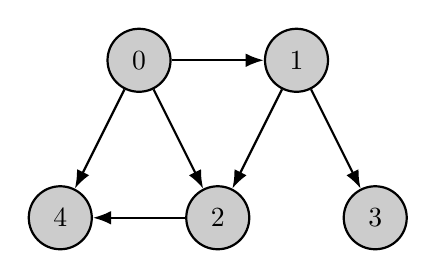
\begin{tikzpicture}[->,sibling distance=10em,line width=0.8pt,-Latex,
    every node/.style = {shape=circle, rounded corners,
        draw, align=center,minimum size=0.8cm,line width=0.8pt,
    fill=black!20}]]
    \node (a) at (1,  0) {0};
    \node (c) at (3,  0) {1};
    \node (d) at (4, -2) {3};
    \node (e) at (2, -2) {2};
    \node (f) at (0, -2) {4};

    \path[every node/.style={font=\sffamily\small}]
        (a) edge node[right] {} (c)
        (a) edge node[right] {} (e)
        (a) edge node[right] {} (f)
        (c) edge node[right] {} (d)
        (c) edge node[right] {} (e)
        (e) edge node[right] {} (f);
\end{tikzpicture}
\end{document}
